\cleardoubleevenemptypage

\begin{figure*}[ht!]
  \centering
  \vspace{-4.6cm}
  \centerline{
    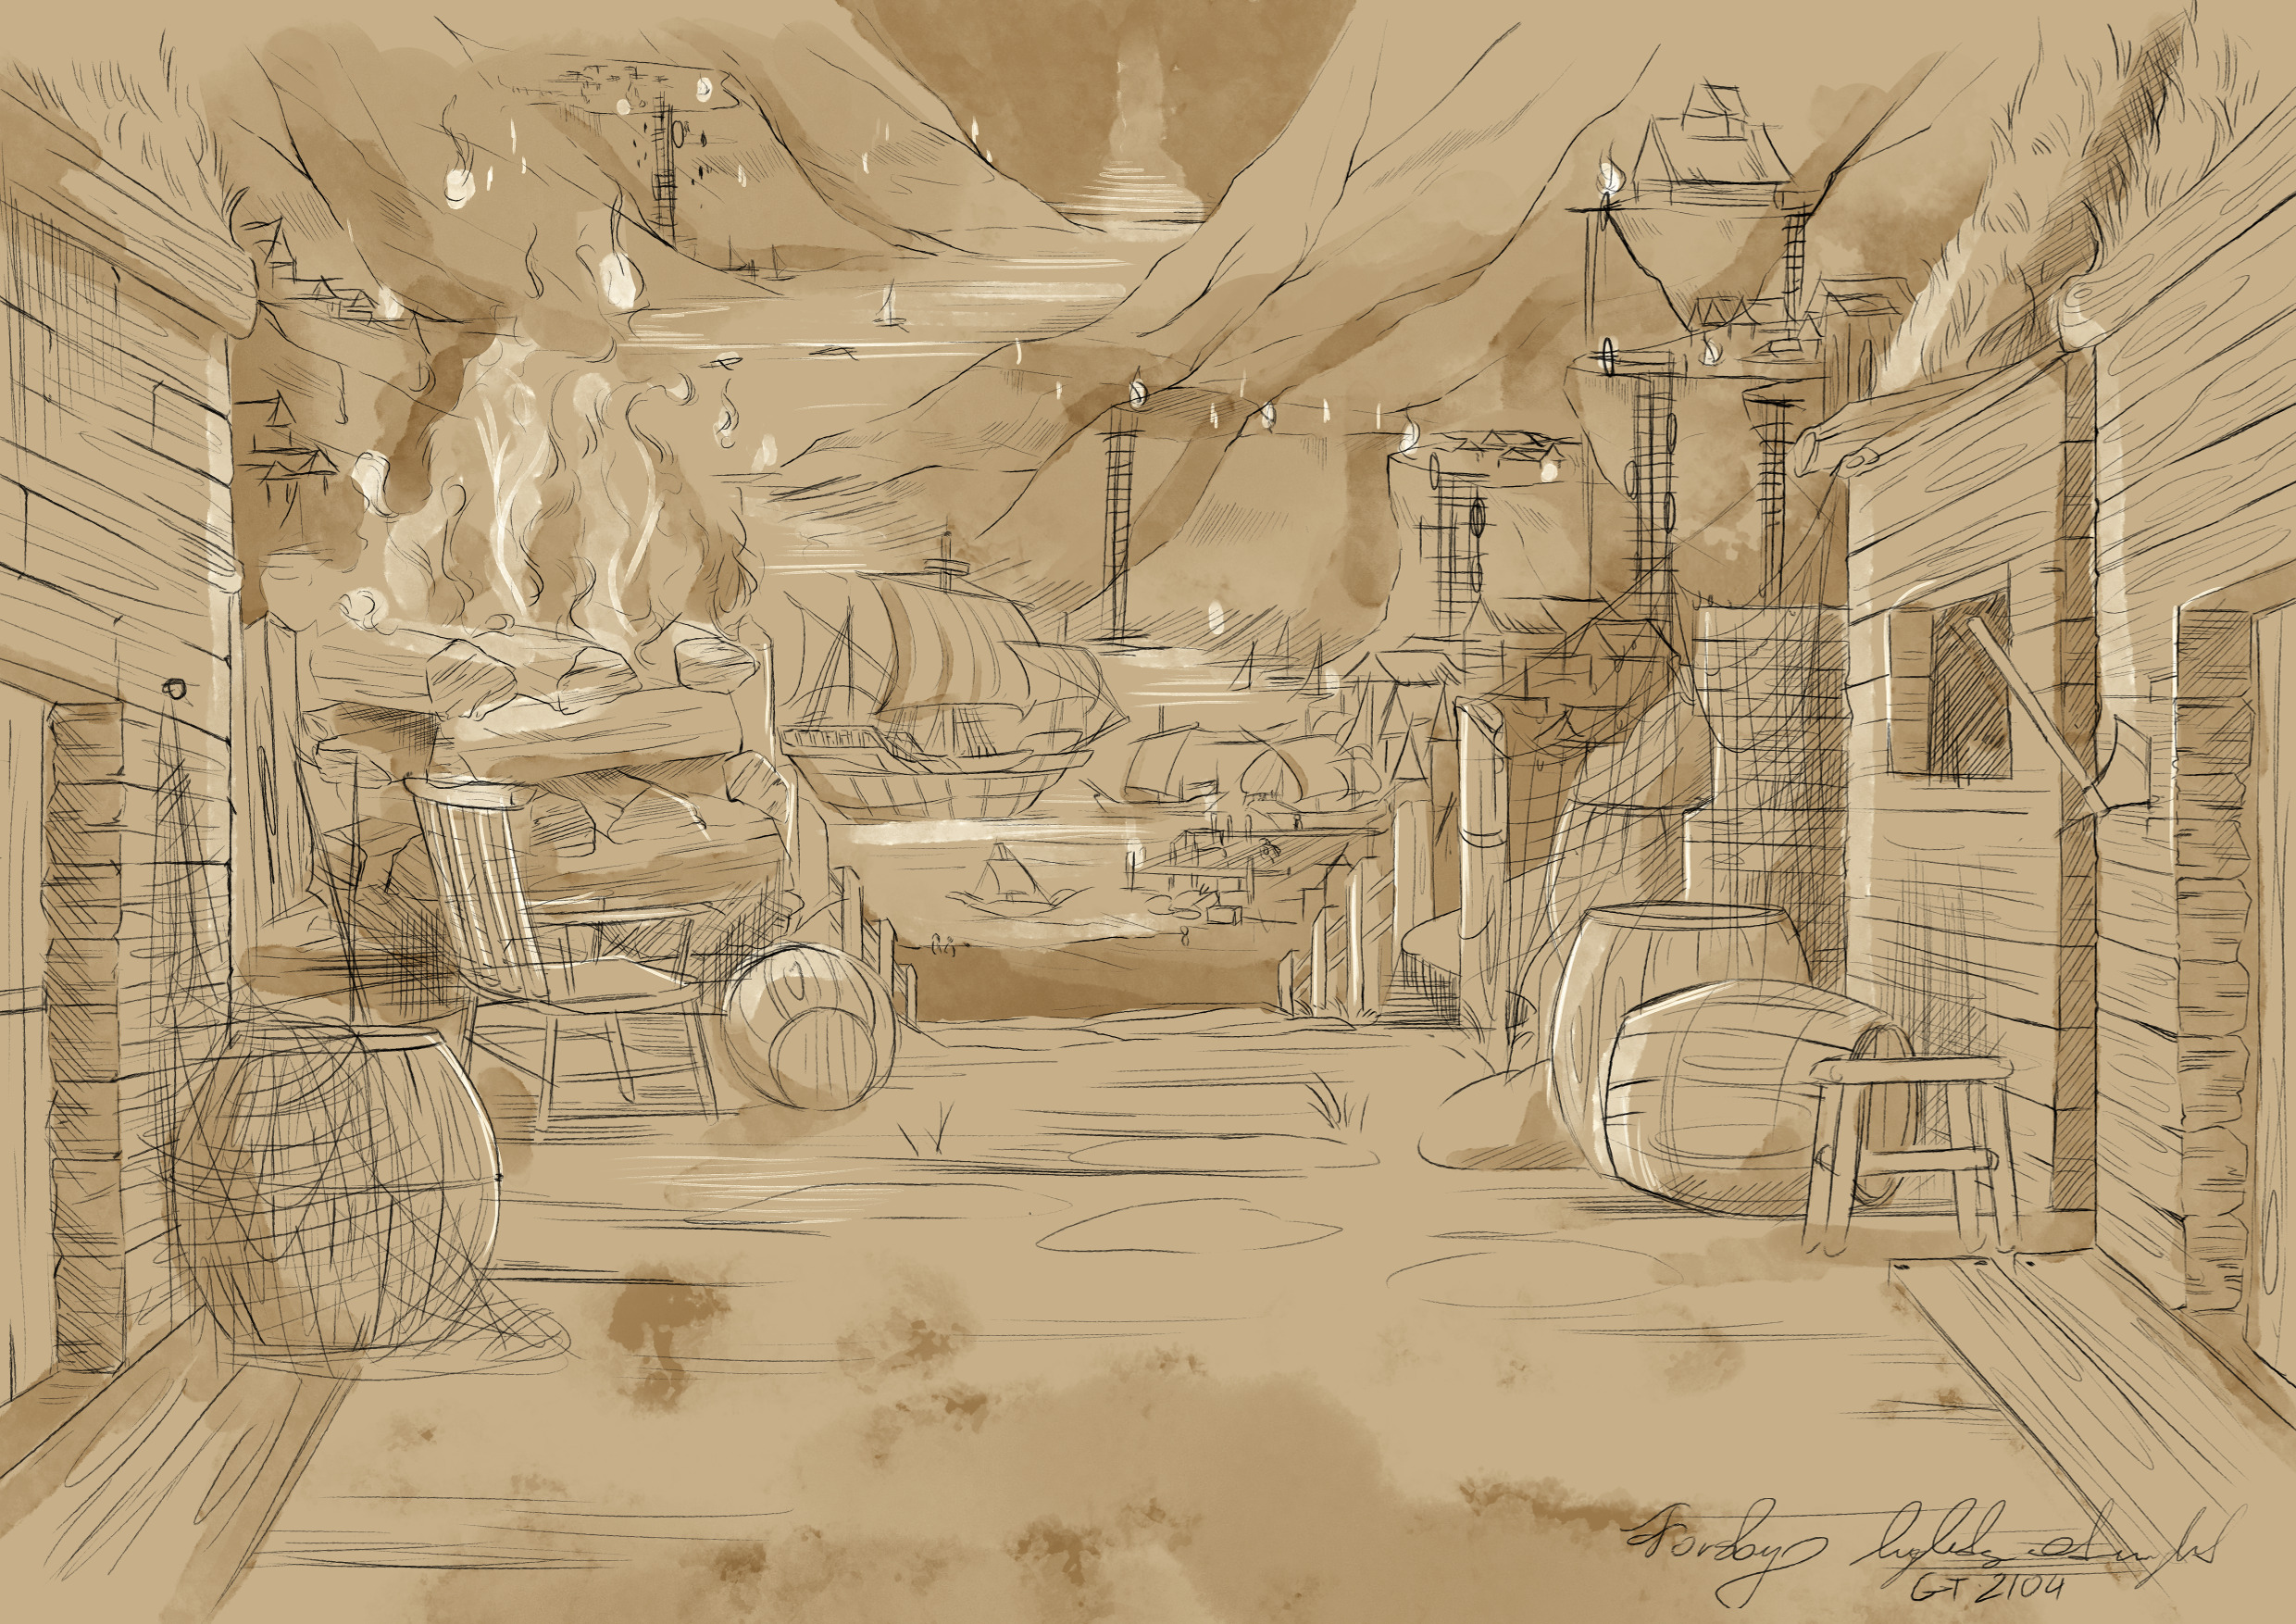
\includegraphics[width=\paperwidth,keepaspectratio]{media/forsby-a3-sm.png}
  }
  \par
  View from the Midway tavern, GT:2104
\end{figure*}

\vspace{-0.5cm}

\begin{infobox}{City Kingdom of Forsby}
  \begin{subfigure}[t]{\textwidth}
    \centering
    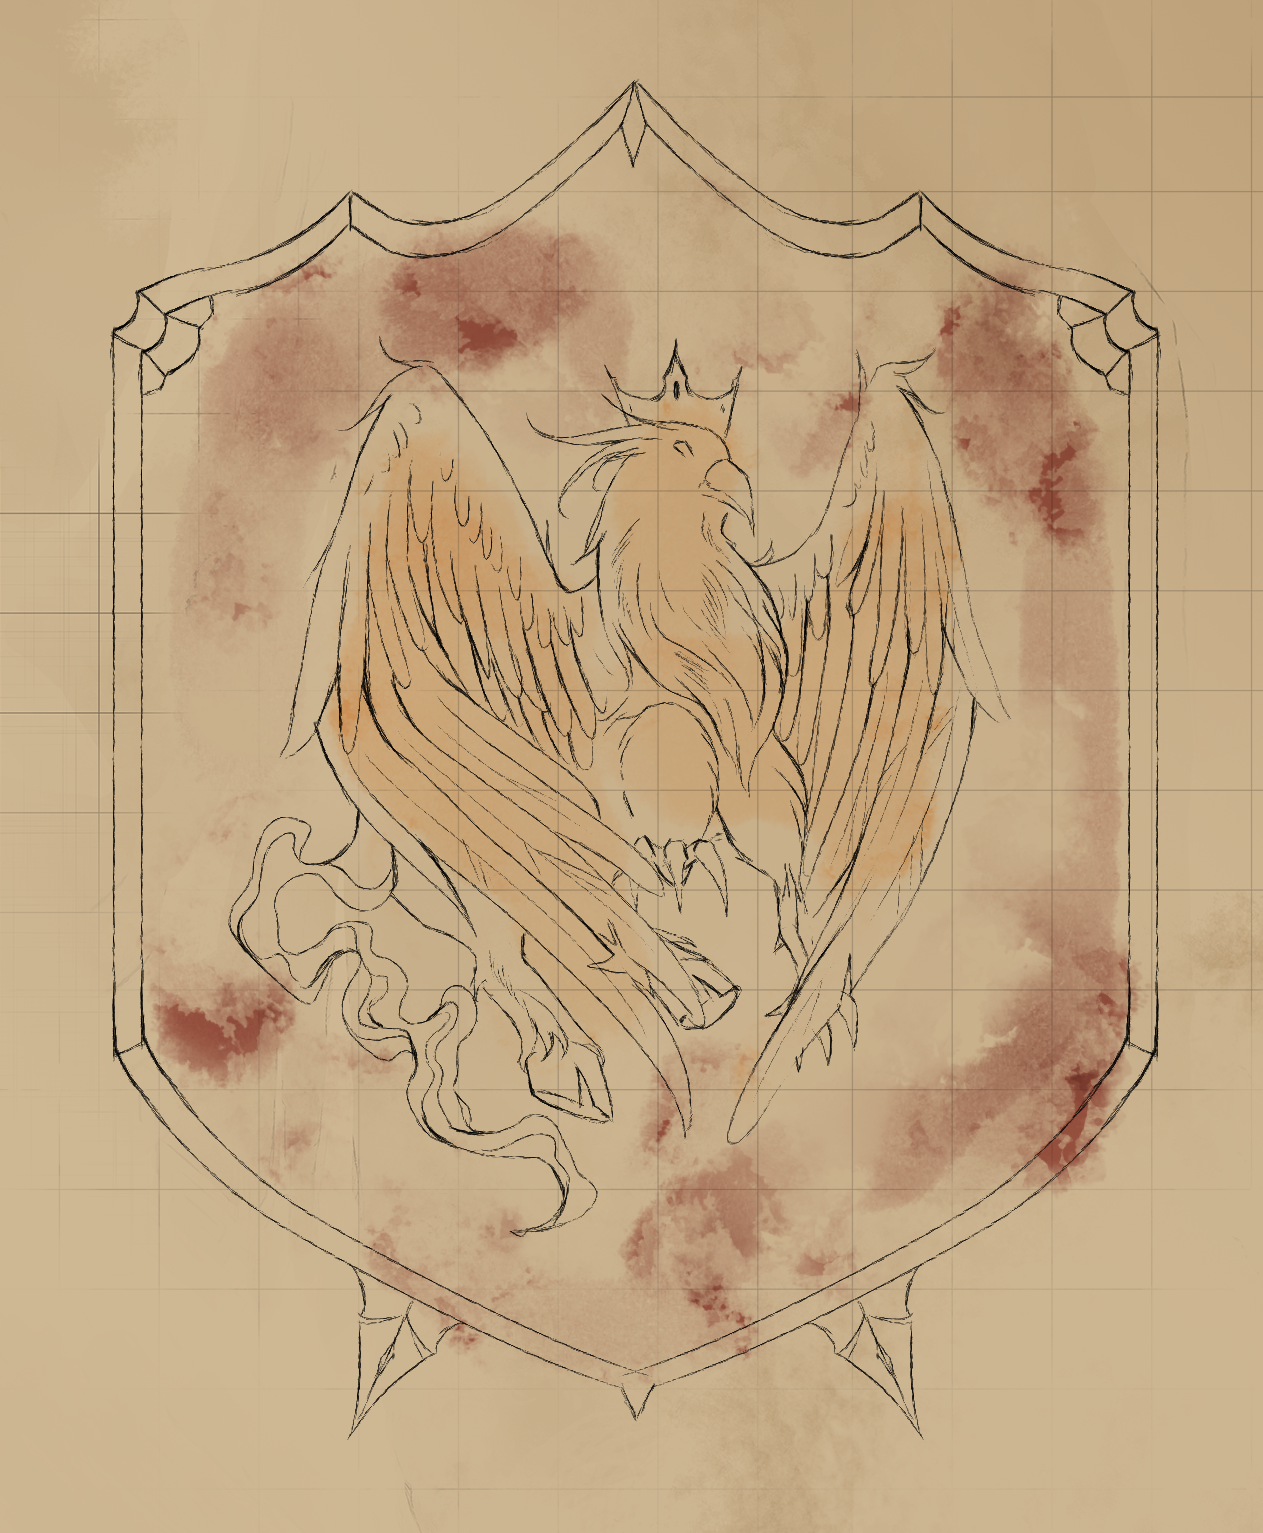
\includegraphics[width=0.20\linewidth]{media/forsby_banner_sm.png}
  \end{subfigure}
  \vspace{-1.0cm}
  \begin{multicols}{2}
    \begin{itemize}[label={},noitemsep,leftmargin=0.0cm,topsep=0pt]
      \infoboxitem{Location}{Western shores of North \nameref{sec:Goltir}}
      \infoboxitem{Languages}{Reatham (dialect), Teranim, Doresh}
      \infoboxitem{Government}{Absolute Monarchy}
      \infoboxitem{Major Religions}{\nameref{sec:Lor}, \nameref{sec:Old Ways}
        \nameref{sec:Order}
      }
      \infoboxitem{Demographics}{est. 150,000 $km^2$, pop. est. 12 million
      }
      \infoboxitem{Non Grata}{devils, druids, monstrous races, undead without
        any citizenship
      }
      \infoboxitem{Magic}{soul magic, necromancy, summoning, and calling
        outlawed; divine, psionic and arcane magic require permits
      }
      \infoboxitem{Slavery}{outlawed, indentured servitude as punishment for
        criminals, signer of the \nameref{sec:Vonir Accord}
      }
      \infoboxitem{Special Laws}{\nameref{sec:Gorgons} must suppress their
        powers while in public
      }
      \infoboxitem{Notable Organisations}{headquarters of the
        \nameref{sec:Magistrata Arcanum}, \nameref{sec:House Ranian},
        \nameref{sec:Ror-Aram Trading Corporation}, headquarters of the
        \nameref{sec:Holy Church of Aleaste}
      }
      \infoboxitem{POI}{Castle Forchtenberg, Midway Point, the
        \nameref{sec:Pit}, cathedral of \nameref{sec:Lor}, public library,
        university of the Magistrata Arcanum with dragon teleporter, Forchtenberg
        park, recreational area alongside the river Hafon, knight's temple of Aleaste
      }
    \end{itemize}
  \end{multicols}
\end{infobox}

\FloatBarrier
\clearpage

\subsection{Forsby}
\label{sec:Forsby}

\aren{You can tell someone hails from Forsby from the first word that comes
  out of their mouth.}

The city kingdom of \emph{Forsby} (``city of streams''), also known as
\emph{Forchtenberg} in local dialect, was founded in \emph{GT:1148}, and
resides on the western shores of the continent of \hyperref[sec:Goltir]{North
Goltir}. Up until the devil siege, it was one of the biggest and wealthiest
of the city kingdoms.

Forsby's banner depicts a yellow hippogriff within a shield, upon a red
backdrop. A crown with three tips rests upon the hippogriff's head.

\subsubsection{The City}

Forsby castle was built the edge of a narrow fjord, upon white cliffs, giving
it a grant view of the sea. The noble district, common area, as well as the
main square lie in a semi circle around the main castle up on the cliff
itself. The kingdom's lands extend beyond the wall of the city, as it owns
large areas of fertile farmlands in the Toralian Highlands. The largest
bulk of the kingdoms populations lives on top of the cliffs, either in the
common area around the castle or as farmers in the highlands. The northern
lands are fed by the river \emph{Hafon}, and the kingdom uses the river both
for its fertile farmland further east, as well as for fresh drinking water
within the city. Any waste from the city is also carried down river into the
sea. The Hafon river crashes into the bay at the southern side of the cliff.

At the bottom of the white cliffs lies the city kingdom's harbour district. The
harbour district is completely built on wooden and stone stilts and pillars,
and fills out most of the cliffs basin. The surrounding cliffs that encircle
the harbour act like a natural defensive barrier, forcing all incoming ships
to pass a narrow passage into the city's harbour. The cliff itself is adorned
with many grand statues holding fire cauldrons, light houses, temples, as well
as fortifications and make the city a truly magnificent view when approaching
it from the sea. Many people, especially workers, traders, and sailors also
live in the extensive harbour district.

Several elevators, both for people and goods, connect the upper cliff side
with the harbour down below. There are also many stairs, passages, and small
caves that were hewn into the cliff side that allow people to travel between
the upper city and the lower harbour. Some people also live in smaller houses
hewn into the cliff side. A well known, and old tavern called ``Midway Point''
rests halfway between the harbour and the castle.

Lying in the northern parts of Goltir, Forsby experiences harsh and cold
winters, and mild summers. While the soil is fertile, only the strongest crops
grow in this harsher climate. Forsby is surrounded by lush and ancient pine
forests, as well as ample farmland.

\subsubsection{Population}

Forsby, and its surrounding outlying villages, is home to roughly 12 million
people, of which most (58\%) are human. Closely followed by deepkin (16\%)
and the elven races (12\%), dwarves (8\%) and various half races (4\%) and
others (2\%) such as Diarim and Umgeher.

Common male names are: Alois, Anton, Bogdan, Boris, Dejan, Emil, Ferdinand,
Gal, Gustaf, Janos (Jan), Johannes (Johan, Hannes), Robert, Miklos, Nikola
(Nikolaus, Nikolai), Radek, Soma, Simon, Viktor, Walter

Common female names are: Anna, Abigel, Bianka, Brana, Elisabeth (Elsa, Lisa),
Elena, Emma, Emelie (Amalie), Helene, Johanna, Magda, Melinda, Nada (Nadia,
Nadezhda), Pauline (Line, Lina), Rosalie (Rosa), Sobena, Vera, Vesna

\subsubsection{Pit}
\label{sec:Pit}

But Forsby also has a darker and secretive side. Beneath the main castle and
noble district, deep with the cliff side, lies the aqueduct that transports
the waste down into the sea. It is simply referred to as the \emph{pit}.
Although a vast and dangerous sewer complex, many people and creatures call
its many levels their home. Existence of the pit is an open secret, and many
entrances to it can be found across the cliff side and in the harbour for
Forsby. Strategies on how to handle the pit, and its denizens, vary greatly
from monarch to monarch. But most follow the ``out-of-sight'' strategy: As
long as no criminal activity bleeds to the surface the pit is free to do as
it pleases.

The upper level houses a vast bazaar and active criminal underworld, where
everything and everyone can be bought for the right price. It also houses a
large tavern and inn, called the ``Golden Mug'' that serves as a neutral
ground for the pit's many criminal gangs. Citizens do sometimes wander the
bazaar, and apart from pickpockets, the bazaar is a save place to do both
illegal and legal business. Most criminal gangs now that scarring away
customers by openly fighting and feuding at the bazaar is counter to their
business' wealth and prosperity.

The lower levels are a different beast however. They are mainly uncharted, and
often house creatures that would not be welcome on the surface. Sightings of
feral vampires, sentient flesh golem butchers, devils, and hags have been
reported in the lower depths of the pit.

\subsubsection{Culture}

Although Forsby has a long standing tradition of chivalry and nobility, the
general population is well aware of the hypocrisy by not moving against the
criminal underworld of the \emph{pit}. The average citizen is nevertheless
proud of the ancient history of the city, its wealth and that a long line of
just kings and queens have lead the kingdom to become one the most powerful on
the planet. Forsby is world-renowned for its arcane academy - called the
\nameref{sec:Magistrata Arcanum} - which has produced many fine and
outstanding wizards. As well as for its public schools that teach any children
within the city and kingdom, and give them a basic education for free.

The people of Forsby are known as stubborn, patriotic, determined but hard
working to achieve their goals. They are well recognised by their rather
cryptic dialect of the common language called \emph{Reatham}. The city itself
used to be open to every civilised race, but after knights of Lor took hold,
they outlawed monstrous races, and devils from entering the city.

The most worshipped religions of Forsby \nameref{sec:Forun},
\nameref{sec:Lor}, but also \nameref{sec:Aria} with the less noble elements
that work and live in the \emph{pit}. Many holidays of Forun are also national
holidays and celebrations in Forsby, including the harvest festival and the
festival of day of candles.

\subsubsection{Nobility}

The city kingdom of Forsby has a long standing tradition of noble
families that have been in charge of the cities affairs for several hundred
years. Their names carry weight even outside the borders of the city, and
they are well established in other city kingdoms across the globe.

The three major families are \emph{Hohenhaus}, \emph{Burgau} and \emph{Csaky}
who have, in turn, ruled the city since its foundation. Hohenhaus is embedded
in the church of \nameref{sec:Lor}, and many of its members are knights,
scribes and priests within the holy church of Lor. Burgau runs the kingdoms
financial sector, and owns many of the artisans, smithies and crafting
guilds. While Csaky is deeply embedded in the city's \nameref{sec:Magistrata
  Arcanum}, and many of its patrons and leaders are well respected wizards,
arcane scholars and arcane craftsmen. These three houses have been known to
feud and fight amongst each other, yet still they share one common goal: the
survival and prosperity of the kingdom.

While these three vie for the throne, there are several smaller houses of
nobility that control smaller aspects of the city: House \emph{Forholm} runs
the cities trading company and shipping docks, and have been known to do
business with the shadier aspects of the \emph{pit}. The House of
\emph{Lemberg} operates most of the kingdom's farms outside of the city, and
are vital to the city's self sustainability in terms of food and agricultural
products.

\subsubsection{Slavery}

The city kingdom of Forsby outlawed slavery, but remains the right to force
criminals into indentured servitude. However this servitude is not extended
to private individuals, and criminals work off their debts and crimes in public
service instead. However the city is a signer of the \nameref{sec:Vonir Accord},
and thus does not free slaves of other signer states, and accepts other slave
owners right to the property.

\subsubsection{Devil Siege}
\label{sec:Devil Siege}

\aren{It is hard to find someone that was not a part or at least affected by
  the war against the devils.}

In MI:2017 the city came under siege by a large force of devils who besieged
the city by land and by sea. After the initial wave of attackers were driven
back by the local knights of the \nameref{sec:Order}, \nameref{sec:Lor}, city
guards and mages of the tower; a second, even bigger wave began laying siege
on the city. During the initial weeks of the siege many of the surrounding
villages of the kingdom were destroyed and its inhabitants were either killed,
or had to flee into the city. The kingdom was both besieged from the sea by
infernal ships made of steel and iron, as well as from several devil legions
by land.

As the siege dragged on for weeks, many more allies of Forsby - such as
\nameref{sec:Hraglund}, \nameref{sec:Norbury}, \nameref{sec:Helmarnock} or
\nameref{sec:Tredegar} sent reinforcements. After the elves and halflings of
Avenfjord joined the coalition, the defenders created a military base on the
Silver Isles to jointly attempt to break the sea embargo that cut off
Forsby. In the last moments before the assault, even \nameref{sec:Morkan} joined
with a small fleet war ships. Although the steel ships of the devils were
superior, the vast amount of ships and men raised by the coalition broke
through the sea embargo. The coalition lost many ships and men, and only a
handful of vessels made it to the harbour of Forsby. Even though the elves and
halflings of \nameref{sec:Avenfjord} promised ships, none of their ships or
troops made it to the rally point to aid Forsby.

During the time of the siege a group of heroes recruited by the coalition
secured the help of an elder white dragon named \emph{Northwind}. Northwind,
and his army of monstrous creatures proved invaluable to defeat the armies of
the devils. It is unknown what happened to the leader of the devils, though
the prevailing theory is that he abandoned the battle after the dragon and its
army came to aid the city.

The siege lasted for almost 7 months, and was formally declared won in the
second month of MI:2018. The reigning monarch \emph{Johann Paul of Hohenhaus}
died during the final battle of the siege, and his son \emph{Johann II of
  Hohenhaus} became king. The dragon remained nearby, and - although most of
his minions perished - it still holds a vast political influence in Forsby.

The siege left all affected kingdoms in a weakened state. Many men and women
perished during the siege, and towns and hamlets were left empty or without
a significant amount of their population. Many ships were lost and the
struggle to rebuild became an arms race among the city kingdoms and larger
baronies. But the siege proved that all kingdoms could work together when
faced with a common enemy. The outcome of the war soured relationship between
Forsby and Avenfjord, who failed to provide promised resources and ships. It
also lead to hostility toward anyone perceived to be a devil sympathiser or
spy, causing massive extra-judicial persecutions and killings of perceived
devil worshippers and summoners, as well as \nameref{sec:Tieflings}.

It is unknown why the devils attempted to invade Forsby, but many, including
the church of Lor, suspected the mage's guild. The guild however denies any
responsibility or knowledge of the attack prior to the siege. Still the
nobility, and the church of Lor, interfered into the guild's business, banning
several practises, such as necromancy and heavily restricting others such as
conjuration, and especially summoning.

\subsubsection{Relations}

Forsby holds good relations with most city kingdoms, even with
\nameref{sec:Morkan}. The kingdom of Forsby is a signer of the
\nameref{sec:Vonir Accord}. The city holds a large church of \nameref{sec:Lor}
and its nobility is tightly interwoven with the church.
